\documentclass[letter,12pt]{article}
\usepackage[paperheight=27.94cm,paperwidth=21.59cm,bindingoffset=0in,left=3cm,right=2.0cm, top=3.5cm,bottom=2.5cm, headheight=200pt, headsep=1.0\baselineskip]{geometry}
\usepackage{graphicx,lastpage}
\usepackage{upgreek}
\usepackage{censor}
\usepackage[spanish,es-tabla]{babel}
\usepackage{pdfpages}
\usepackage{tabularx}
\usepackage{graphicx}
\usepackage{adjustbox}
\usepackage{xcolor}
\usepackage{colortbl}
\usepackage{rotating}
\usepackage{multirow}
\usepackage[utf8]{inputenc}
\usepackage{float}
\usepackage{hyperref}

\renewcommand{\tablename}{Tabla}
\usepackage{fancyhdr}
\pagestyle{fancy}

\usepackage{listings}
\usepackage{caption}

\definecolor{darkerGreen}{rgb}{0.0, 0.5, 0.0}


% Define counter for code listings


\newcounter{codecount}
\renewcommand{\thecodecount}{\arabic{codecount}}

% Redefine caption for listings
\DeclareCaptionFormat{myformat}{Código \thecodecount: #3}
\captionsetup[lstlisting]{format=myformat, labelformat=empty}

% Definición del lenguaje JavaScript
\lstdefinelanguage{JavaScript}{
  keywords={break, case, catch, continue, debugger, default, delete, do, else, finally, for, function, if, in, instanceof, new, return, switch, this, throw, try, typeof, var, void, while, with, let, const, of},
  keywordstyle=\color{blue}\bfseries,
  ndkeywords={class, export, boolean, throw, implements, import, this},
  ndkeywordstyle=\color{blue}\bfseries,
  identifierstyle=\color{black},
  sensitive=false,
  comment=[l]{//},
  morecomment=[s]{/*}{*/},
  commentstyle=\color{darkerGreen}\ttfamily,
  stringstyle=\color{red}\ttfamily,
  morestring=[b]',
  morestring=[b]"
}

% Definición del lenguaje Dockerfile
\lstdefinelanguage{Dockerfile}{
  keywords={FROM, COPY, RUN, CMD, ENTRYPOINT, VOLUME, ADD, WORKDIR, ARG, ENV, EXPOSE, LABEL, STOPSIGNAL, USER, HEALTHCHECK, ONBUILD, SHELL},
  keywordstyle=\color{blue}\bfseries,
  identifierstyle=\color{black},
  sensitive=true,
  comment=[l]{#},
  commentstyle=\color{darkerGreen}\ttfamily,
  stringstyle=\color{red}\ttfamily,
  morestring=[b]',
  morestring=[b]"
}

% Estilo general para los códigos
\lstdefinestyle{mystyle}{
  basicstyle=\ttfamily\small,
  backgroundcolor=\color[rgb]{0.95, 0.95, 0.95},
  numberstyle=\tiny\color{gray},
  numbersep=5pt,
  stepnumber=1,
  frame=single,
  breaklines=true,
  showstringspaces=false,
  captionpos=b,
  numbers=left,
  morekeywords={*,...},
  postbreak=\mbox{\textcolor{cyan}{$\hookrightarrow$}\space}  
}

\lstset{style=mystyle}



%
\begin{document}
%
   \title{\Huge{Informe Laboratorio 5}}

   \author{\textbf{Sección 1} \\  \\Alumno Omar Marca \\ e-mail: omar.marca@mail.udp.cl}
          
   \date{Junio de 2024}

   \maketitle

   \newpage
   
   \tableofcontents
 
  \newpage
  

\section*{Descripción de actividades}
\addcontentsline{toc}{section}{Descripción de actividades}
Para este último laboratorio, nuestro informante ya sabe que puede establecer un medio seguro sin un intercambio previo de una contraseña, gracias al protocolo diffie-hellman. El problema es que ahora no sabe si confiar en el equipo con el cual establezca comunicación, ya que las credenciales de usuario pueden haber sido divulgadas por algún soplón.\\

Para el presente laboratorio deberá:

\begin{itemize}
    \item Crear 4 contenedores en Docker o Podman, donde cada uno tendrá el siguiente SO:
        Ubuntu 16.10, Ubuntu 18.10, Ubuntu 20.10 y Ubuntu 22.10 a los cuales se llamarán C1, C2, C3 y C4 respectivamente.\\
        El equipo con Ubuntu 22.10 también será utilizado como S1.
        
    \item  Para cada uno de ellos, deberá instalar el cliente openSSH disponible en los repositorios de apt, y para el equipo S1 deberá también instalar el servidor openSSH.

    \item En S1 deberá crear el usuario \textquotedblleft\textbf{prueba}\textquotedblright con contraseña \textquotedblleft\textbf{prueba}\textquotedblright, para acceder a él desde los clientes por el protocolo SSH.
    
    \item En total serán 4 escenarios, donde cada uno corresponderá a los siguientes equipos:
    \begin{itemize}
        \item C1 $\rightarrow$ S1
        \item C2 $\rightarrow$ S1
        \item C3 $\rightarrow$ S1
        \item C4 $\rightarrow$ S1
    \end{itemize}
\end{itemize}

Pasos:

\begin{enumerate}
\item Para cada uno de los 4 escenarios, deberá capturar el tráfico generado por cada conexión con el server. A partir de cada handshake, deberá analizar el patrón de tráfico generado por cada cliente y adicionalmente obtener el HASSH que lo identifique. De esta forma podrá obtener una huella digital para cada cliente a partir de su tráfico. Cada HASSH deberá compararlo con la base de datos HASSH disponible en el módulo de TLS, e identificar si el hash obtenido corresponde a la misma versión de su cliente.\\\\
Indique el tamaño de los paquetes del flujo generados por el cliente y el contenido asociado a cada uno de ellos. Indique qué información distinta contiene el escenario siguiente (diff incremental). El objetivo de este paso es identificar claramente los cambios entre las distintas versiones de ssh.\\

\newpage

\item Para poder identificar que el usuario efectivamente es el informante, éste utilizará una versión única de cliente. ¿Con qué cliente SSH se habrá generado el siguiente tráfico?

\begin{figure}[ht]
    \centering
    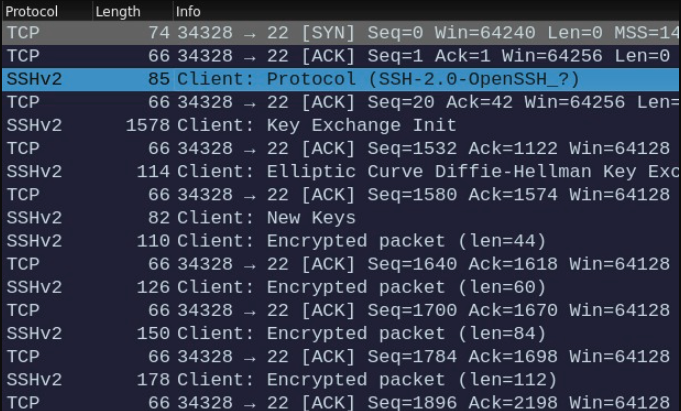
\includegraphics[width=1\linewidth]{Desarrollo/trafico.png}
    \caption{Tráfico generado del informante}
    \label{fig:trafico}
\end{figure}

Replique este tráfico generado en la imagen. Debe generar el tráfico con la misma versión resaltada en azul. Recuerde que toda la información generada es parte del sw, por lo tanto usted puede modificar toda la información.

\item Para que el informante esté seguro de nuestra identidad, nos pide que el patrón del tráfico de nuestro server también sea modificado, hasta que el Key Exchange Init del server sea menor a 300 bytes. Indique qué pasos realizó para lograr esto.

\begin{figure}[ht]
    \centering
    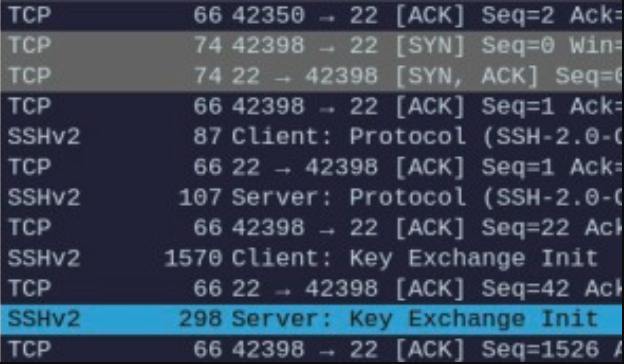
\includegraphics[width=1\linewidth]{Desarrollo/exchange.png}
    \caption{Captura del Key Exchange}
    \label{fig:exchange}
\end{figure}

\end{enumerate}

\clearpage

\section{Desarrollo (Parte 1)}

\subsection{Códigos de cada Dockerfile}

A continuación se muestran los códigos usados en cada dockerfile para automatizar el proceso de instalación de imagenes dentro de lso contenedores en los códigos \ref{code:C1}, \ref{code:C2}, \ref{code:C3}, \ref{code:C4}.

\subsubsection{C1}

\refstepcounter{codecount}\label{code:C1}
\begin{lstlisting}[language=Dockerfile, caption={C1}]
FROM ubuntu:16.10

COPY sources.list /etc/apt/

RUN apt-get update
RUN apt-get install -y openssh-client openssh-server

# Para que el contenedor siga en ejecucion
ENTRYPOINT ["tail", "-f", "/dev/null"]
\end{lstlisting}

\subsubsection{C2}

\refstepcounter{codecount}\label{code:C2}
\begin{lstlisting}[language=Dockerfile, caption={C2}]
FROM ubuntu:18.10

COPY sources.list /etc/apt/

RUN apt-get update
RUN apt-get install -y openssh-client openssh-server

# Para que el contenedor siga en ejecucion
ENTRYPOINT ["tail", "-f", "/dev/null"]
\end{lstlisting}

\subsubsection{C3}

\refstepcounter{codecount}\label{code:C3}
\begin{lstlisting}[language=Dockerfile, caption={C3}]
FROM ubuntu:20.10

COPY sources.list /etc/apt/

RUN apt-get update
RUN apt-get install -y openssh-client openssh-server

# Para que el contenedor siga en ejecucion
ENTRYPOINT ["tail", "-f", "/dev/null"]
\end{lstlisting}

\subsubsection{C4/S1}

\refstepcounter{codecount}\label{code:C4}
\begin{lstlisting}[language=Dockerfile, caption={C4}]
FROM ubuntu:22.10

COPY entrypoint.sh .
COPY sources.list /etc/apt/

RUN apt-get update
RUN apt-get install -y tshark

# Creacion de usuario prueba
ARG USER=prueba
ARG PASS="prueba"
RUN useradd -m -s /bin/bash $USER && echo "$USER:$PASS" | chpasswd

# Instalacion de SSH
RUN apt-get install -y openssh-client openssh-server

RUN chmod +x entrypoint.sh

ENTRYPOINT ["./entrypoint.sh"]
\end{lstlisting}

\clearpage

\subsection{Creación de las credenciales para S1}

Para conectar por SSH de un contenedor a otro, se declara en la imagen C4\_S1 que el cliente se pueda autenticar con el usuario ''prueba" y la contraseña ''prueba" tal y como se muestra a continuación en el fragmento de código \ref{code:credenciales} del Dockerfile.

\refstepcounter{codecount}\label{code:credenciales}
\begin{lstlisting}[language=Dockerfile, caption={Fragmento del Dockerfile en el código \ref{code:C4} de c4\_s1 con las credenciales. }]
# Creacion de usuario prueba
ARG USER=prueba
ARG PASS="prueba"
RUN useradd -m -s /bin/bash $USER && echo "$USER:$PASS" | chpasswd
\end{lstlisting}


\subsection{Tráfico generado por C1, detallando tamaño paquetes del flujo y el HASSH respectivo (detallado)}

Al abrir la captura de paquetes que se envían entre c1 y c4\_s1, se aprecia la siguiente figura \ref{fig:trafico_c1}:

\begin{figure}[ht]
    \centering
    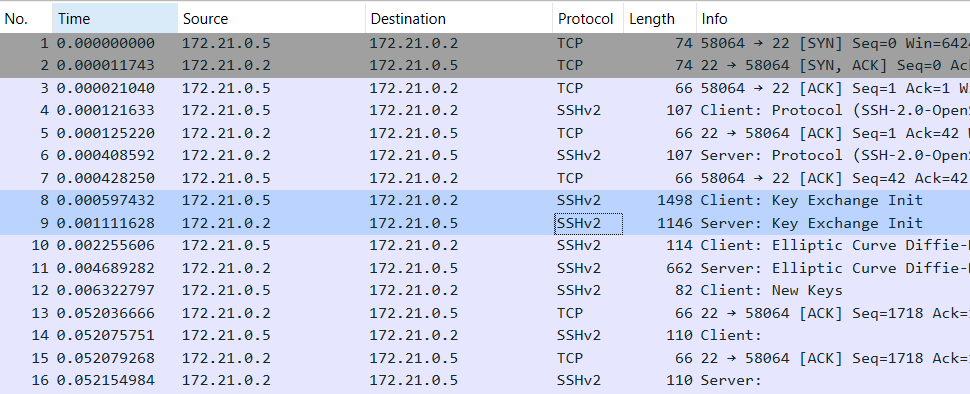
\includegraphics[width=1\linewidth]{Images/parte1/trafico_c1.png}
    \caption{Tráfico generado por C1}
    \label{fig:trafico_c1}
\end{figure}

La IP 172.21.0.2 corresponde al contenedor c4\_s1 (servidor) y 172.21.0.5 al contenedor c1 (cliente). En esta figura \ref{fig:trafico_c1} se puede el handshake que se hace entre paquetes en donde se puede ver lo siguiente:

\begin{enumerate}
    \item Fila 1: El cliente le envía un SYN al servidor.
    
    \item Fila 2: El servidor le envía un SYN al cliente.

    \item Fila 3: El cliente le envía un ACK al servidor.

    \item Fila 5: El servidor le envía un ACK al cliente.

    \item Fila 7: El cliente le envía un ACK al servidor.

    \item Fila 8 y 9: Da aviso a que el intercambio de llaves ha sido iniciado para ambas máquinas.

    \item Fila 13: Por ultimo, El servidor le envía un ACK al cliente.

\end{enumerate}

La información que se envían los paquetes en los ACK son números con valores muy altos los cuales son utilizados para establecer una comunicación segura entre cliente y servidor. Para entender de mejor manera como funciona, se adjunta \href{https://www.cloudflare.com/learning/ssl/what-happens-in-a-tls-handshake/}{en este enlace}, información sobre el funcionamiento de TLS Handshake.\\
\\
El tamaño de los paquetes ACK varía, no obstante en la fila 8 y 9 el tamaño solo varía según la versión de ubuntu que se está utilizando. En este caso tiene un tamaño de 1498 bytes para el cliente y 1146 para el servidor.


\subsection{Tráfico generado por C2, detallando tamaño paquetes del flujo y el HASSH respectivo (detallado)}

Tal y como se describió en la sección 1.3, para el contenedor c2 es exactamente lo mismo solamente que cambia el tamaño del paquete de la fila 8 correspondiente al cliente en la siguiente figura \ref{fig:textoplanoC2}:

\begin{figure}[ht]
    \centering
    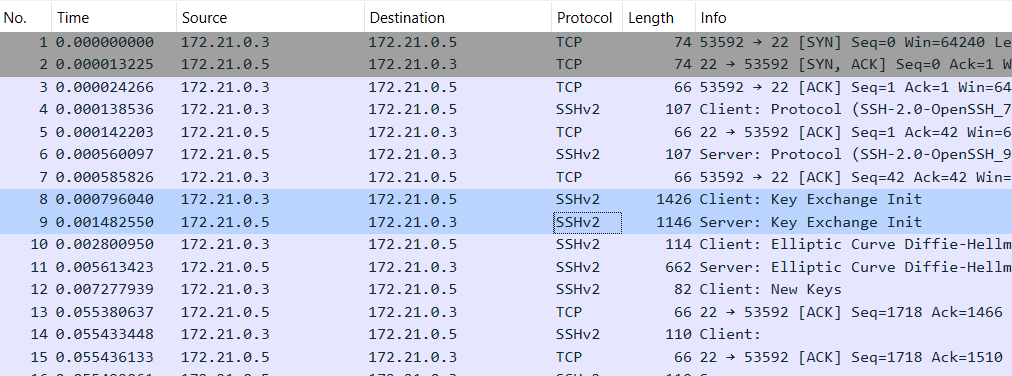
\includegraphics[width=1\linewidth]{Images/parte1/trafico_c2.png}
    \caption{Tráfico generado por C2}
    \label{fig:trafico_c2}
\end{figure}

Entonces, el tamaño del paquete de la linea 8 en la figura \ref{fig:textoplanoC2} es de 1426 bytes.

\clearpage

\subsection{Tráfico generado por C3, detallando tamaño paquetes del flujo y el HASSH respectivo (detallado)}

Tal y como se describió en la sección 1.3, para el contenedor c3 es exactamente lo mismo solamente que cambia el tamaño del paquete de la fila 8 correspondiente al cliente en la siguiente figura \ref{fig:textoplanoC3}:


\begin{figure}[ht]
    \centering
    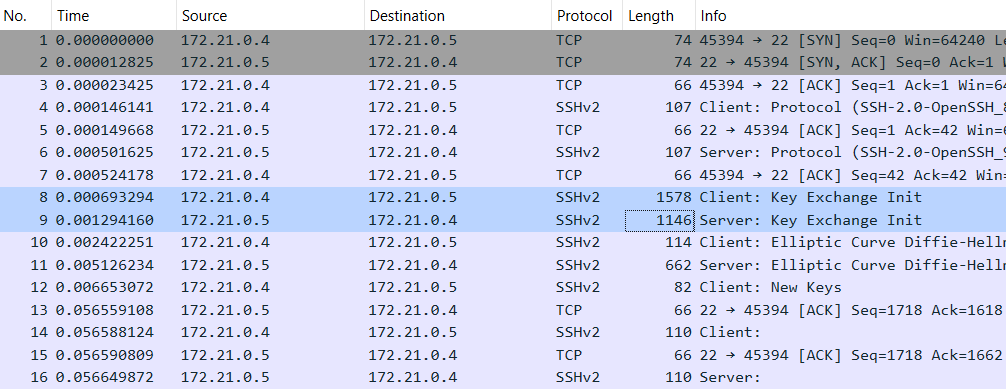
\includegraphics[width=1\linewidth]{Images/parte1/trafico_c3.png}
    \caption{Tráfico generado por C3}
    \label{fig:trafico_c3}
\end{figure}

Entonces, el tamaño del paquete de la linea 8 en la figura \ref{fig:textoplanoC3} es de 1578 bytes.

\clearpage

\subsection{Tráfico generado por C4 (iface lo), detallando tamaño paquetes del flujo y el HASSH respectivo (detallado)}

Tal y como se describió en la sección 1.3, para el contenedor c4 es exactamente lo mismo solamente que cambia el tamaño del paquete de la fila 12 correspondiente al cliente (que es el mismo contenedor) y que la conexión SSH se la está haciendo a si mismo en la siguiente figura \ref{fig:textoplanoC4}:



\begin{figure}[ht]
    \centering
    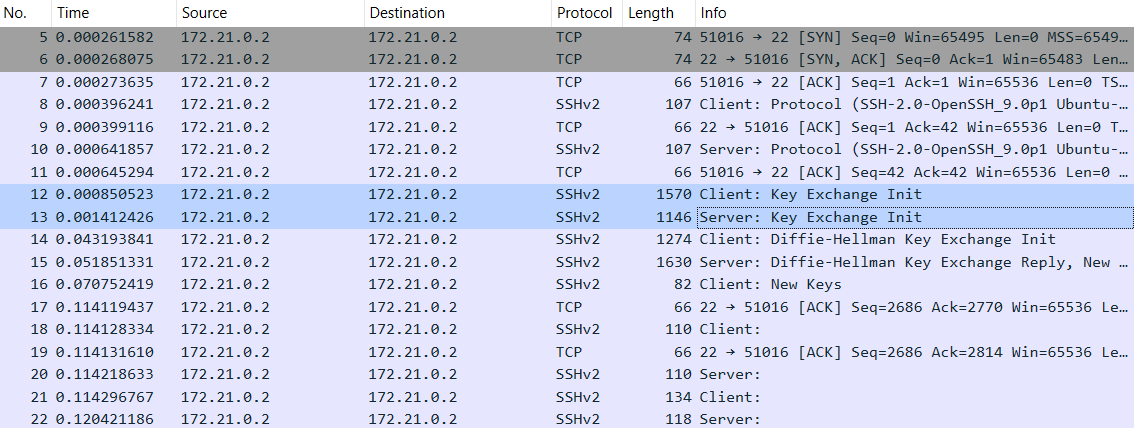
\includegraphics[width=1\linewidth]{Images/parte1/trafico_c4.png}
    \caption{Tráfico generado por C4}
    \label{fig:trafico_c4}
\end{figure}

Entonces, el tamaño del paquete de la linea 12 en la figura \ref{fig:textoplanoC4} es de 1570 bytes.



\subsection{Compara la versión de HASSH obtenida con la base de datos para validar si el cliente corresponde al mismo}




\clearpage

\subsection{Tipo de información contenida en cada uno de los paquetes generados en texto plano}

Dentro de la información de cada paquete se tienen las siguientes secciones del campo SSH Protocol:

\begin{itemize}
    \item Packet Length: Indica el tamaño del campo SSH protocol.

    \item Padding Length: Indica el tamaño del padding aplicado para el campo de SSH protocol.

    \item Hey Exchange: Indica el mensaje y los algoritmos utilizados cuando se hace el intercambio de llaves entre cliente y servidor.

    \item Padding string: Indica el padding utilizado.

    
\end{itemize}

\subsubsection{C1}

A continuación se muestra en la figura \ref{fig:textoplanoC1} el campo SSH con la información de c1.


\begin{figure}[ht]
    \centering
    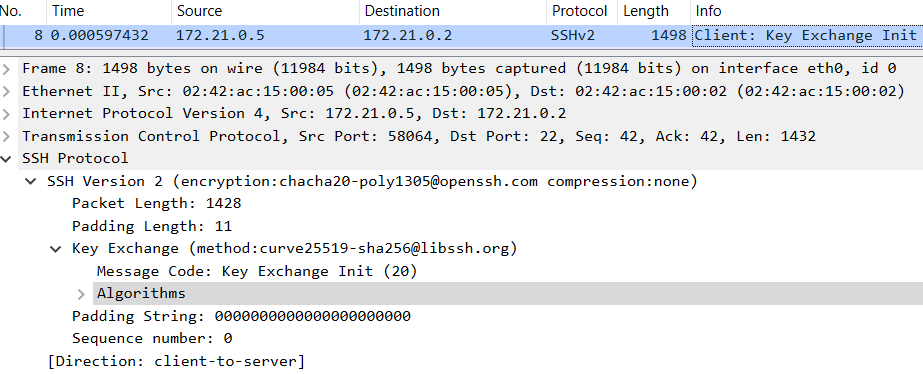
\includegraphics[width=1\linewidth]{Images/parte1/textoplano/textoplanoC1.png}
    \caption{Tipo de información contenida en los paquetes de C1}
    \label{fig:textoplanoC1}
\end{figure}


\clearpage

\subsubsection{C2}


A continuación se muestra en la figura \ref{fig:textoplanoC2} el campo SSH con la información de c2.

\begin{figure}[ht]
    \centering
    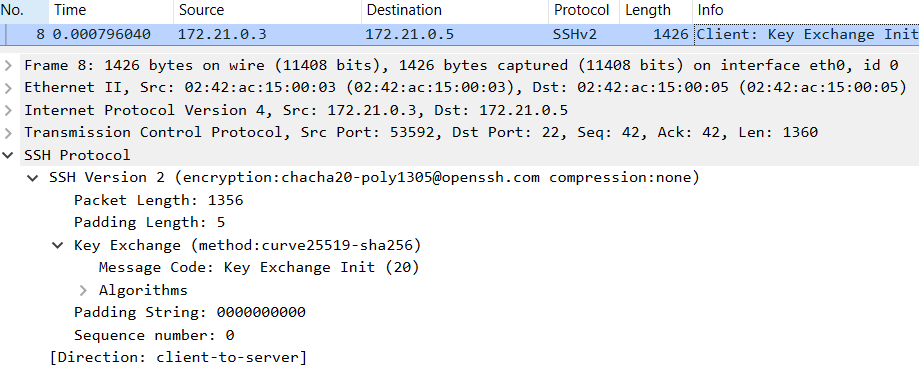
\includegraphics[width=1\linewidth]{Images/parte1/textoplano/textoplanoC2.png}
    \caption{Tipo de información contenida en los paquetes de C2}
    \label{fig:textoplanoC2}
\end{figure}



\subsubsection{C3}

A continuación se muestra en la figura \ref{fig:textoplanoC3} el campo SSH con la información de c3.
\begin{figure}[ht]
    \centering
    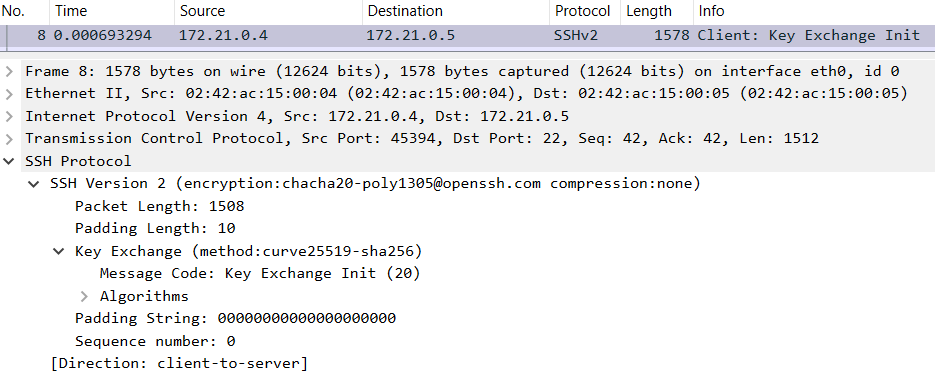
\includegraphics[width=1\linewidth]{Images/parte1/textoplano/textoplanoC3.png}
    \caption{Tipo de información contenida en los paquetes de C3}
    \label{fig:textoplanoC3}
\end{figure}

\clearpage

\subsubsection{C4/S1}

A continuación se muestra en la figura \ref{fig:textoplanoC4} el campo SSH con la información de c4.

\begin{figure}[ht]
    \centering
    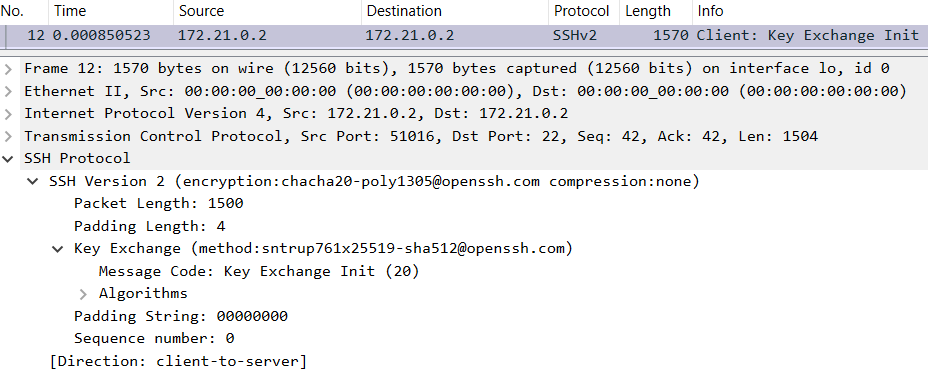
\includegraphics[width=1\linewidth]{Images/parte1/textoplano/textoplanoC4.png}
    \caption{Tipo de información contenida en los paquetes de C4}
    \label{fig:textoplanoC4}
\end{figure}


\subsection{Diferencia entre C1 y C2}

Observando la figura \ref{fig:textoplanoC1} y \ref{fig:textoplanoC2}, se puede apreciar a simple vista que las diferencias radican en el tamaño de los paquetes y el tamaño del padding utilizado.\\
\\
Por otra parte, también cambia el método utilizado que en el caso de c1 es ''curve25519-sha256@libssh.org'' y para c2 es ''curve25519-sha256''\\
\\
Al analizar la captura, cambia las coockies de ambos paquetes y el hassh.

\subsection{Diferencia entre C2 y C3}

Observando la figura \ref{fig:textoplanoC2} y \ref{fig:textoplanoC3}, se puede apreciar a simple vista que las diferencias radican en el tamaño de los paquetes y el tamaño del padding utilizado.\\
\\
Al analizar la captura, cambia las coockies de ambos paquetes y el hassh.

\subsection{Diferencia entre C3 y C4}

Observando la figura \ref{fig:textoplanoC3} y \ref{fig:textoplanoC4}, se puede apreciar a simple vista que las diferencias radican en el tamaño de los paquetes y el tamaño del padding utilizado.\\
\\
Por otra parte, también cambia el método utilizado que en el caso de c3 es ''curve25519-sha256'' y para c4\_s1 es ''sntrup761x25519-sha512@openssh.com''\\
\\
Al analizar la captura, cambia las coockies de ambos paquetes y el hassh.


\newpage

\section{Desarrollo (Parte 2)}

\subsection{Identificación del cliente SSH con versión \textquotedblleft?\textquotedblright}

Para todos los casos, el cliente SSH siempre será el que se quiere conectar a un servidor en este caso c4\_s1. Es por ello que a continuación se muestra en la figura \ref{fig:clienteC1}, \ref{fig:clienteC2}, \ref{fig:clienteC3} y \ref{fig:clienteC4}, como se identifica el cliente SSH en los paquetes por Wireshark.

\begin{figure}[ht]
    \centering
    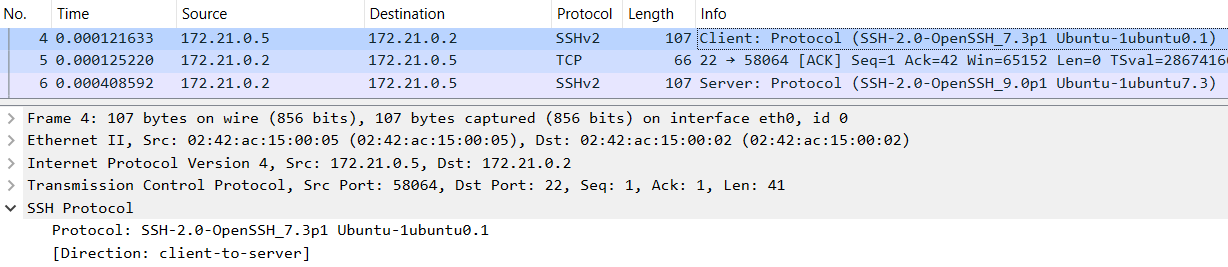
\includegraphics[width=1\linewidth]{Images/parte2/clienteSSH/clienteC1.png}
    \caption{Cliente SSH C1}
    \label{fig:clienteC1}
\end{figure}

Como se puede apreciar en la figura \ref{fig:clienteC1}, la versión del cliente c1 es ''SSH-2.0-OpenSSH\_7.3p1 Ubuntu-1ubuntu0.1"

\begin{figure}[ht]
    \centering
    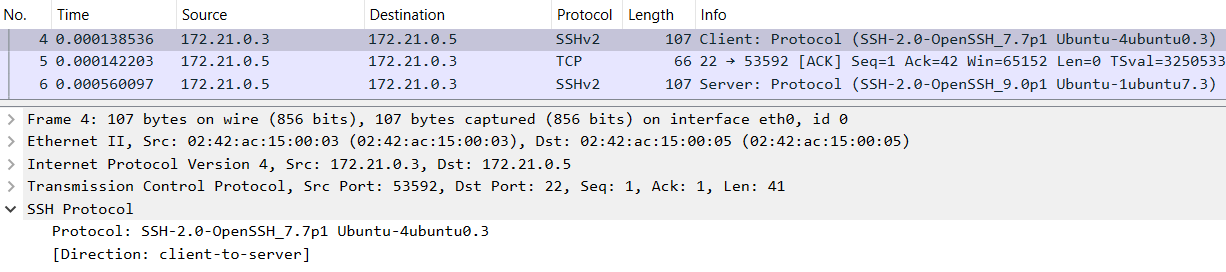
\includegraphics[width=1\linewidth]{Images/parte2/clienteSSH/clienteC2.png}
    \caption{cliente SSH C2}
    \label{fig:clienteC2}
\end{figure}

En la figura \ref{fig:clienteC2}, se muestra que la versión del cliente c2 es ''SSH-2.0-OpenSSH\_7.7p1 Ubuntu-4ubuntu0.3"



\begin{figure}[ht]
    \centering
    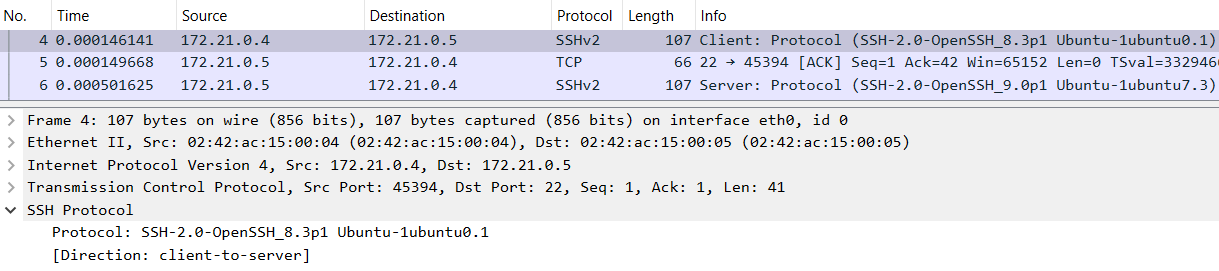
\includegraphics[width=1\linewidth]{Images/parte2/clienteSSH/clienteC3.png}
    \caption{cliente SSH C3}
    \label{fig:clienteC3}
\end{figure}

En la figura \ref{fig:clienteC3}, se muestra que la versión del cliente c3 es ''SSH-2.0-OpenSSH\_8.3p1 Ubuntu-1ubuntu0.1"




\begin{figure}[ht]
    \centering
    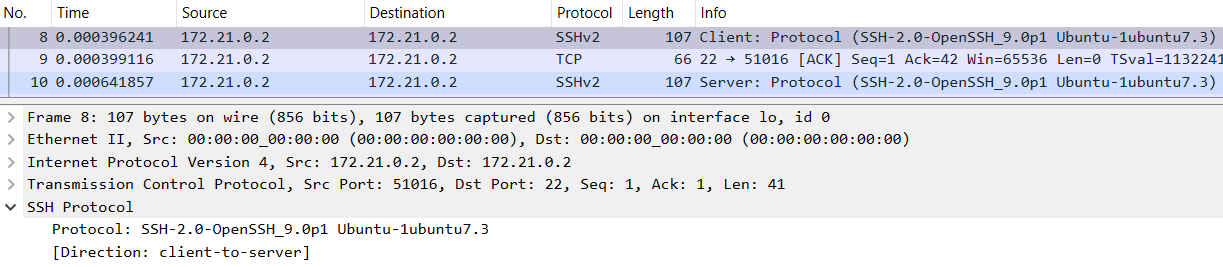
\includegraphics[width=1\linewidth]{Images/parte2/clienteSSH/clienteC4.png}
    \caption{cliente SSH C4}
    \label{fig:clienteC4}
\end{figure}

Notar que en la figura \ref{fig:clienteC4} el cliente SSH es el mismo servidor SSH puesto a que en el caso del contenedor c4\_s1 se esta conectando a si mismo. Por otra parte, su versión corresponde a SSH-2.0-OpenSSH\_9.0p1 Ubuntu-1ubuntu7.3


\subsection{Replicación de tráfico al servidor (paso por paso)}

Para replicar el servidor se tiene el siguiente dockerfile en el código \ref{code:Dockerfilenuevo}:


\refstepcounter{codecount}\label{code:Dockerfilenuevo}
\begin{lstlisting}[language=Dockerfile, caption={Dockerfile nuevo para c4\_s1}]
FROM ubuntu:22.10

# Copiar scripts y archivos necesarios
COPY entrypoint.sh .
COPY sources.list /etc/apt/

# Actualizar los repositorios y instalar dependencias necesarias
RUN apt-get update && \
    apt-get install -y build-essential zlib1g-dev libssl-dev libpam0g-dev libselinux1-dev wget  
    ## apt-get install -y tshark

# Crear usuario prueba
ARG USER=prueba
ARG PASS="prueba"
RUN useradd -m -s /bin/bash $USER && echo "$USER:$PASS" | chpasswd

# Descargar el codigo fuente de OpenSSH
RUN wget https://cdn.openbsd.org/pub/OpenBSD/OpenSSH/portable/openssh-9.0p1.tar.gz && \
    tar -xzf openssh-9.0p1.tar.gz

# Modificar el numero de version
RUN cd openssh-9.0p1 && \
    sed -i 's/^#define SSH_VERSION.*/#define SSH_VERSION "OpenSSH_?"/' version.h && \
    ./configure && \
    make && \
    make install

# Hacer el script de entrada ejecutable
RUN chmod +x entrypoint.sh

ENTRYPOINT ["./entrypoint.sh"]

\end{lstlisting}


Luego al corroborar la versión de SSH en la terminal de c4\_s1 se muestra la siguiente figura \ref{fig:sshversion}:

\begin{figure}[ht]
    \centering
    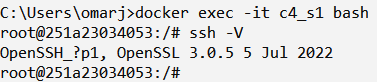
\includegraphics[width=0.6\linewidth]{Images/parte2/sshversion.png}
    \caption{Versión ssh modificada}
    \label{fig:sshversion}
\end{figure}



\clearpage

\section{Desarrollo (Parte 3)}

\subsection{Replicación del KEI con tamaño menor a 300 bytes (paso por paso)}

La documentación de como se hace fue hecha a partir de     \item Explicación Para cambiar el tamaño de los paquetes en SSH por la página de openssh \href{https://www.openssh.com/legacy.html}{este enlace}.

\begin{enumerate}
    \item Se debe ir a la ruta ''etc/ssh/sshd\_config" para modificar el archivo sshd\_config.

    \item Luego en el archivo se debe colocar la siguiente configuración mostrada en el fragmento de código \ref{code:parte3} y luego reiniciar el servicio ssh:

    
\refstepcounter{codecount}\label{code:parte3}
\begin{lstlisting}[language=Dockerfile, caption={Modificación del archivo sshd\_config}]
Ciphers 3des-cbc
MACs hmac-sha1
HostKeyAlgorithms ssh-ed25519
KexAlgorithms diffie-hellman-group1-sha1
\end{lstlisting}

\item Luego se colocar tshark para capturar paquetes, se debe ir a la terminal de otro contenedor (en este caso c3) y producto de que se cambian los algoritmos SSH, se debe colocar el siguiente comando en el código \ref{code:parte3.1}:

\refstepcounter{codecount}\label{code:parte3.1}
\begin{lstlisting}[language=Dockerfile, caption={Terminal de otro contenedor (c3 en este caso)}]
ssh -oKexAlgorithms=+diffie-hellman-group1-sha1 -c 3des-cbc prueba@c4\_s1

\end{lstlisting}

\item Luego de terminar la captura, se podrán apreciar las modificaciones de los tamaños tal y como se muestra en la figura \ref{fig:parte3}:

\begin{figure}[H]
    \centering
    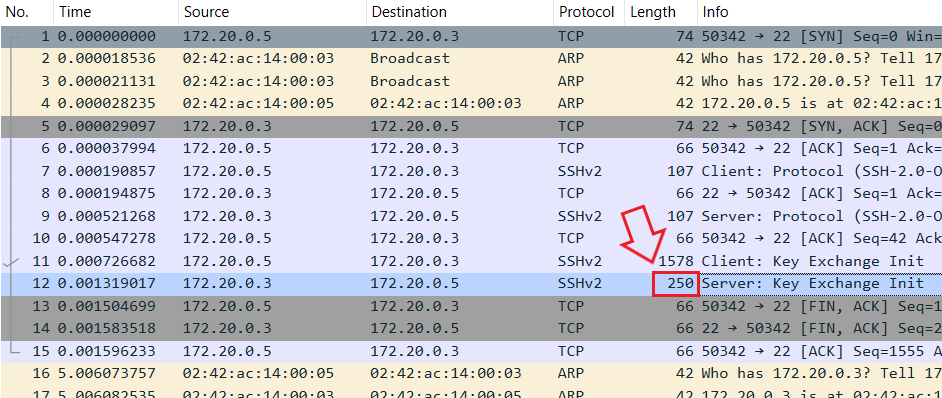
\includegraphics[width=1\linewidth]{Images/parte 3/parte3.png}
    \caption{Paquete con tamaño modificado.}
    \label{fig:parte3}
\end{figure}

El paquete modificado se puede apreciar con un rectángulo rojo siendo apuntado con una flecha.

\end{enumerate}

\clearpage

\section*{Conclusiones y comentarios}

SSH es un herramienta muy util para el acceso de una maquina remota a otra. Es por eso que en esta experiencia se evidencia más información acerca de como trabaja el protocolo SSH dando a entender que utiliza algoritmos como RSA, Diffie-Hellman para el intercambio de claves, curvas elipticas, sha-sha20, entre otros. Es importante conocer el funcionamiento del protocolo SSH debido a su gran uso comercial hoy en día con el acceso remoto de unas maquinas a otras y entender como mantiene la confidencialidad de los datos personales a la hora de compartir información.

\subsection*{Issues}

\begin{enumerate}
    \item \textbf{Issue 1: Permisos para c4\_s1 en su Dockerfile.}

Al momento de intentar iniciar el contenedor c4\_s1, se mostraba un error de permisos al instalar openssh, orl o que para solucionarlo se colocó en su dockerfile el código \ref{code:issue1}

\refstepcounter{codecount}\label{code:issue1}
\begin{lstlisting}[language=Dockerfile, caption={Solución al issue 1}]
RUN chmod +x entrypoint.sh
\end{lstlisting}

Esto lo que hará es otorgarle más permisos al archivo entrypoint.sh.

    \item \textbf{Issue 2: C4 no captura nada en ssh.}

Cuando c4\_s1 se estaba conectando a si mismo mediante ssh, al insertar en el contenedor c4\_s1 el comando del código \ref{code:issue2} en la terminal, no se captura ni se muestra nada.

\refstepcounter{codecount}\label{code:issue2}
\begin{lstlisting}[language=Dockerfile, caption={No captura paquetes a si mismo en c4\_s1}]
tshark -i eth0 -w capture.pcap
\end{lstlisting}

El hecho de que no se capture nada es porque se está conectando a si mismo por la interfaz ''eth0". Para solucionarlo, se cambio la interfaz ''eth0" a la interfaz ''lo" (Loopback) que si captura los paquetes que se envia el contenedor hacia si mismo. El comando quedaría entonces como se muestra en el código \ref{code:issue2.1}

\refstepcounter{codecount}\label{code:issue2.1}
\begin{lstlisting}[language=Dockerfile, caption={Solución al issue 2}]
tshark -i lo -w capture.pcap
\end{lstlisting}


\clearpage

    \item \textbf{Issue 3: Error al usar imágenes de Ubuntu }

Al momento de hacer un docker compose con las distintas versiones de ubuntu, se muestra por terminal el siguiente error mostrado en la figura \ref{fig:issue3} para cada una de las imágenes:

\begin{figure}[ht]
    \centering
    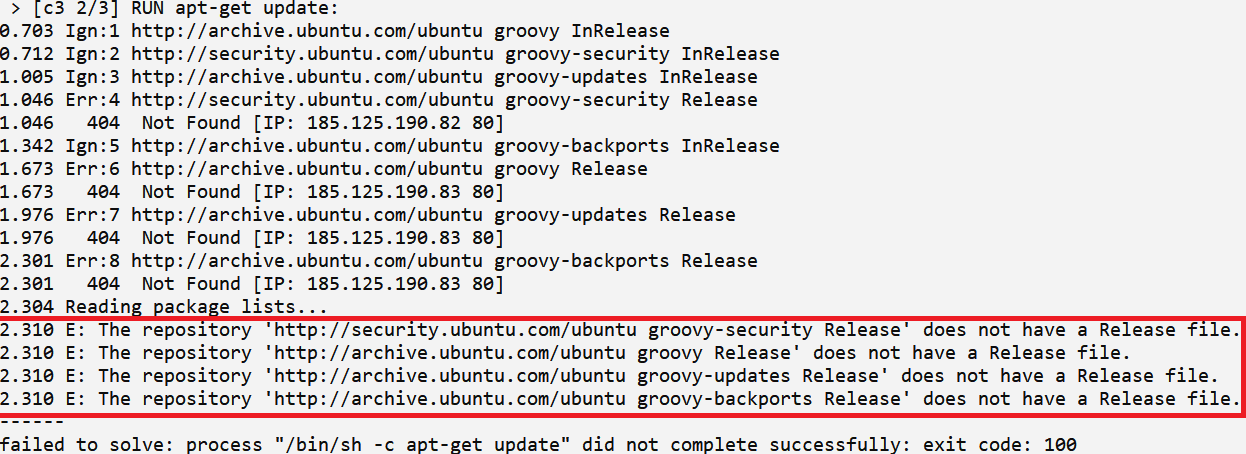
\includegraphics[width=1\linewidth]{Images/issues/issue3.png}
    \caption{Issue 3}
    \label{fig:issue3}
\end{figure}

Este error aparece cuando una versión de ubuntu llegó al final de su vida útil por lo que ya no recibe actualizaciones compatibles. Es por ello que dentro de los foros de soporte de ubuntu \href{https://help.ubuntu.com/community/EOLUpgrades}{en este enlace,} muestran una forma de solucionarlo creando un archivo llamado source.list que contiene lo que se muestra a continuación en el código \ref{code:issue3}

\refstepcounter{codecount}\label{code:issue3}
\begin{lstlisting}[language=Dockerfile, caption={Solución al issue 3}]
## EOL upgrade sources.list
# Required
deb http://old-releases.ubuntu.com/ubuntu/ CODENAME main restricted universe multiverse
deb http://old-releases.ubuntu.com/ubuntu/ CODENAME-updates main restricted universe multiverse
deb http://old-releases.ubuntu.com/ubuntu/ CODENAME-security main restricted universe multiverse
\end{lstlisting}

En donde ''CODENAME" corresponde al nombre de la versión de ubuntu que se está usando. Luego, se debe añadir el siguiente código \ref{code:issue3.1} dentro del dockerfile.


\refstepcounter{codecount}\label{code:issue3.1}
\begin{lstlisting}[language=Dockerfile, caption={Solución al issue 3 en el dockerfile}]
COPY sources.list /etc/apt/
\end{lstlisting}

Luego, se debe hacer esto para cada versión de ubuntu que se quiere instalar.

\clearpage

    \item \textbf{Issue 4: Problema para autenticar usuario por ssh cuando se cambian los tamaños del paquete. }

Al momento de cambiar el tamaño de la llave de los paquetes SSH, se tiene el siguiente error en la figura \ref{fig:issue4} al tratar de establecer la conexión:

\begin{figure}[ht]
    \centering
    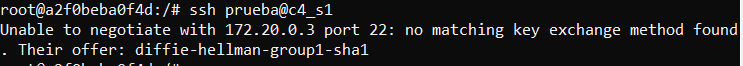
\includegraphics[width=1\linewidth]{Images/issues/issue4.png}
    \caption{Issue 4}
    \label{fig:issue4}
\end{figure}

El error mostrado en la figura \ref{fig:issue4} indica que el cliente SSH y el servidor SSH no comparten un método de intercambio de claves compatible. Esto es debido a que el servidor está usando ''diffie-hellman-group1-sha1" mientras que el cliente está usando otra versión distinta de intercambio de claves. Entonces para adaptar los metodos de intercambio de clave del cliente a los del servidor, se coloca el siguiente código \ref{code:parte3.1}:

\refstepcounter{codecount}\label{code:parte3.1}
\begin{lstlisting}[language=Dockerfile, caption={Terminal de otro contenedor (c3 en este caso)}]
ssh -oKexAlgorithms=+diffie-hellman-group1-sha1 -c 3des-cbc prueba@c4\_s1

\end{lstlisting}

Toda la información para resolver este conflicto se puede observar de mejor manera en la página web de openssh \href{https://www.openssh.com/legacy.html}{en este enlace.}

\end{enumerate}


\clearpage


\subsection*{Referencias}

El apoyo y manejo de algunos comandos se hizo con una combinación entre el uso de herramientas de IA's de código generativas como Chatgpt y Microsoft Bing. Además, se hace uso de la documentación en los siguientes enlaces:



\begin{itemize}
    \item Para hacer funcionar a las versiones de ubuntu anteriores \href{https://help.ubuntu.com/community/EOLUpgrades}{acá}.

    \item Explicación TLS handshake por cloudflare \href{https://www.cloudflare.com/learning/ssl/what-happens-in-a-tls-handshake/}{acá}.

    \item Explicación Para cambiar el tamaño de los paquetes en SSH por la página de openssh \href{https://www.openssh.com/legacy.html}{acá}.



\end{itemize}

\end{document}
